\documentclass[titlepage]{article}
\usepackage[utf8]{inputenc}
\usepackage{amsmath}
\usepackage{tcolorbox}
\usepackage{amssymb}
\usepackage{amsthm}
\usepackage{physics}
\usepackage{empheq}
\usepackage{xcolor}
\usepackage{float}
\usepackage[
top    = 2.50cm,
bottom = 2.50cm,
left   = 2.75cm,
right  = 2.75cm]{geometry}
\usepackage{fancyhdr}
\pagestyle{fancy}
\lhead{Linear algebra 1}
\rhead{EPFL/Alp Ozen}


\makeatletter
\renewcommand*\env@matrix[1][*\c@MaxMatrixCols c]{%
  \hskip -\arraycolsep
  \let\@ifnextchar\new@ifnextchar
  \array{#1}}
\makeatother

\newcommand{\tens}[1]{%
  \mathbin{\mathop{\otimes}\limits_{#1}}%
}

\newtheorem{thm}{Theorem}[subsection]
\newtheorem{property}{Property}
\newtheorem{cor}{Corollary}[subsection]
\newtheorem{prop}{[Proposition]}
\newtheorem{rem}{Remark}[subsection]
\newtheorem{definition}{Definition}[subsection]
\newtheorem{exm}{Example}[subsection]
\numberwithin{equation}{subsection}

%useful macros
\newcommand{\Rn}{\mathbb{R}^n}
\newcommand{\Rm}{\mathbb{R}^m}
\newcommand{\ld}{linearly dependent}
\newcommand{\li}{linearly independent}


\title{\textbf{Linear Algebra 1}}
\author{Alp Ozen}
\date{Fall 2019 - \textcolor{red}{EPFL}}


\begin{document}

\maketitle
\tableofcontents

\clearpage

\section{Linear equations}
\subsection{Basics}

\begin{tcolorbox}
A linear equation is any equation of form:
$a_{1}x_{1}+ ..... + a_{n}x_{n} = b$
where the a are 'scalars' that belong to a field and the x belong to the vector set. 
\end{tcolorbox}

A \textit{system of linear equation}s is simply a collection of linear equations. The solution of this system, if there is any, is an ordered list $(s_{1},...,s_{n})$ where each $s_{i}$ is the value of each $x_{i}$.
\\

A system consisting of 2 unknowns and two linear equations is generally the intersection of two lines on a cartesian plane. Note that the lines may be parallel or even colinear. 
\\

In general, a system will have:
\begin{itemize}
    \item no solution
    \item unique solution
    \item infinite solutions 
\end{itemize}
\\

We may choose to represent a system of linear equations as an \textit{augmented matrix}. A matrix is called n$\times$m if it is of form:
\begin{equation*}
    \begin{bmatrix}
    a_{11} && a{12} &&  ... \\
    a_{21} && a {22}  && ... \\
    \end{bmatrix}
\end{equation*}

\subsection{Solving a linear system}
\subsubsection{Basics}

When solving a system, our goal is to replace each linear equation with an equivalent set(one that has the same solution) and obtain single linear equations which are trivial to solve. 
\\

In solving a system, we use the elementary row operations which are: 

\begin{tcolorbox}
\begin{itemize}
    \item Interchange two rows (or columns).
    \item Multiply each element in a row (or column) by a non-zero number.
    \item Multiply a row (or column) by a non-zero number and add the result to another row (or column).
\end{itemize}
\end{tcolorbox}

Our goal is to transform our matrix into echelon or row reduced echelon form. A matrix is in echelon form if it looks like this: \begin{equation*}
\begin{bmatrix}
    \blacktriangledown &&  \blacktriangle && \blacktriangle \\
    0 && \blacktriangledown && \blacktriangle \\
    0 && 0 && \blacktriangledown

\end{bmatrix}
    
\end{equation*}

Here, each $\blacktriangledown$ and $\blacktriangle$ may take on any value from the set the vector space is defined on. 
\\

To obtain this form, we first arrange our matrix into a form where the row with the least amount of trailing zeros is placed uptop. Then we ensure the \textit{pivot position}(meaning first non-zero entry) has only 0 in its own column. When done, we move on the second row, find the pivot position and repeat. We repeat this process for all rows. 
\\

If we have a system where the number of unknowns exceeds the number of equations, we obtain a parametric solution. Consider this: 

\begin{example}
\begin{equation*}
  \begin{bmatrix}
    1 && 0 &&  -5 && 1 \\
    0 && 1 && 1 && 4 \\
    0 && 0  && 0 && 0 \\
    \end{bmatrix}
\end{equation*}

Which means: 
$$ x_{1} - 5x_{3} = 1$$
$$ x_{2} +  x_{3} = 4$$

Now, we can express both $x_{1}$ and $x_{2}$ in terms of $x_{3}$. We call $x_{1}$ and $x_{2}$ basic variables and $x_{3}$ the free variable. We call $x_{3}$ a free variable as we are free to choose any value for it. 
\end{example}

Most importantly, these are the conditions for row echelon and reduced row echelon form. 

\begin{tcolorbox}
 \textbf{Row echelon form if:}
 \begin{itemize}
     \item all nonzero rows are above zero rows
     \item a leading entry is the right column of a leading entry above it
     \item all entries in a column below a leading entry are 0
 \end{itemize}
 \textbf{Reduced row echelon also if:}
 \begin{itemize}
     \item leading entry in each nonzero row is 1
     \item the entries in the column of the leading entry are 0
 \end{itemize}
\end{tcolorbox}
\\ 

To obtain reduced row echelon form, starting from the lowest row, the terms in the column with the leading term are made zero and the leading term scaled to 1. We repeat this process. 
\\

As a general remark, we obtain the following.

\begin{thm}
A system is consistent iff, the rightmost column has no pivot. More simply, iff the lowest row is not of the form: 
\begin{bmatrix}
    0 && 0 \dots && b
\end{bmatrix}
where b is nonzero. 
\end{thm}
\\

A common confusion when solving a linear system is why the Gaussian algorithm works? To help answer this, the idea is to visualize a Cartesian plane with two random lines intersecting. Now, there can be multiple lines that intersect at the same point. But the intersection of something like $x=2$ and $y=5$ is obviously $(2,5)$ and requires less effort to solve. Thus, we try to replace our equations with those that are easier to solve and have the same solution set. 

\begin{figure}[h]
    \centering
    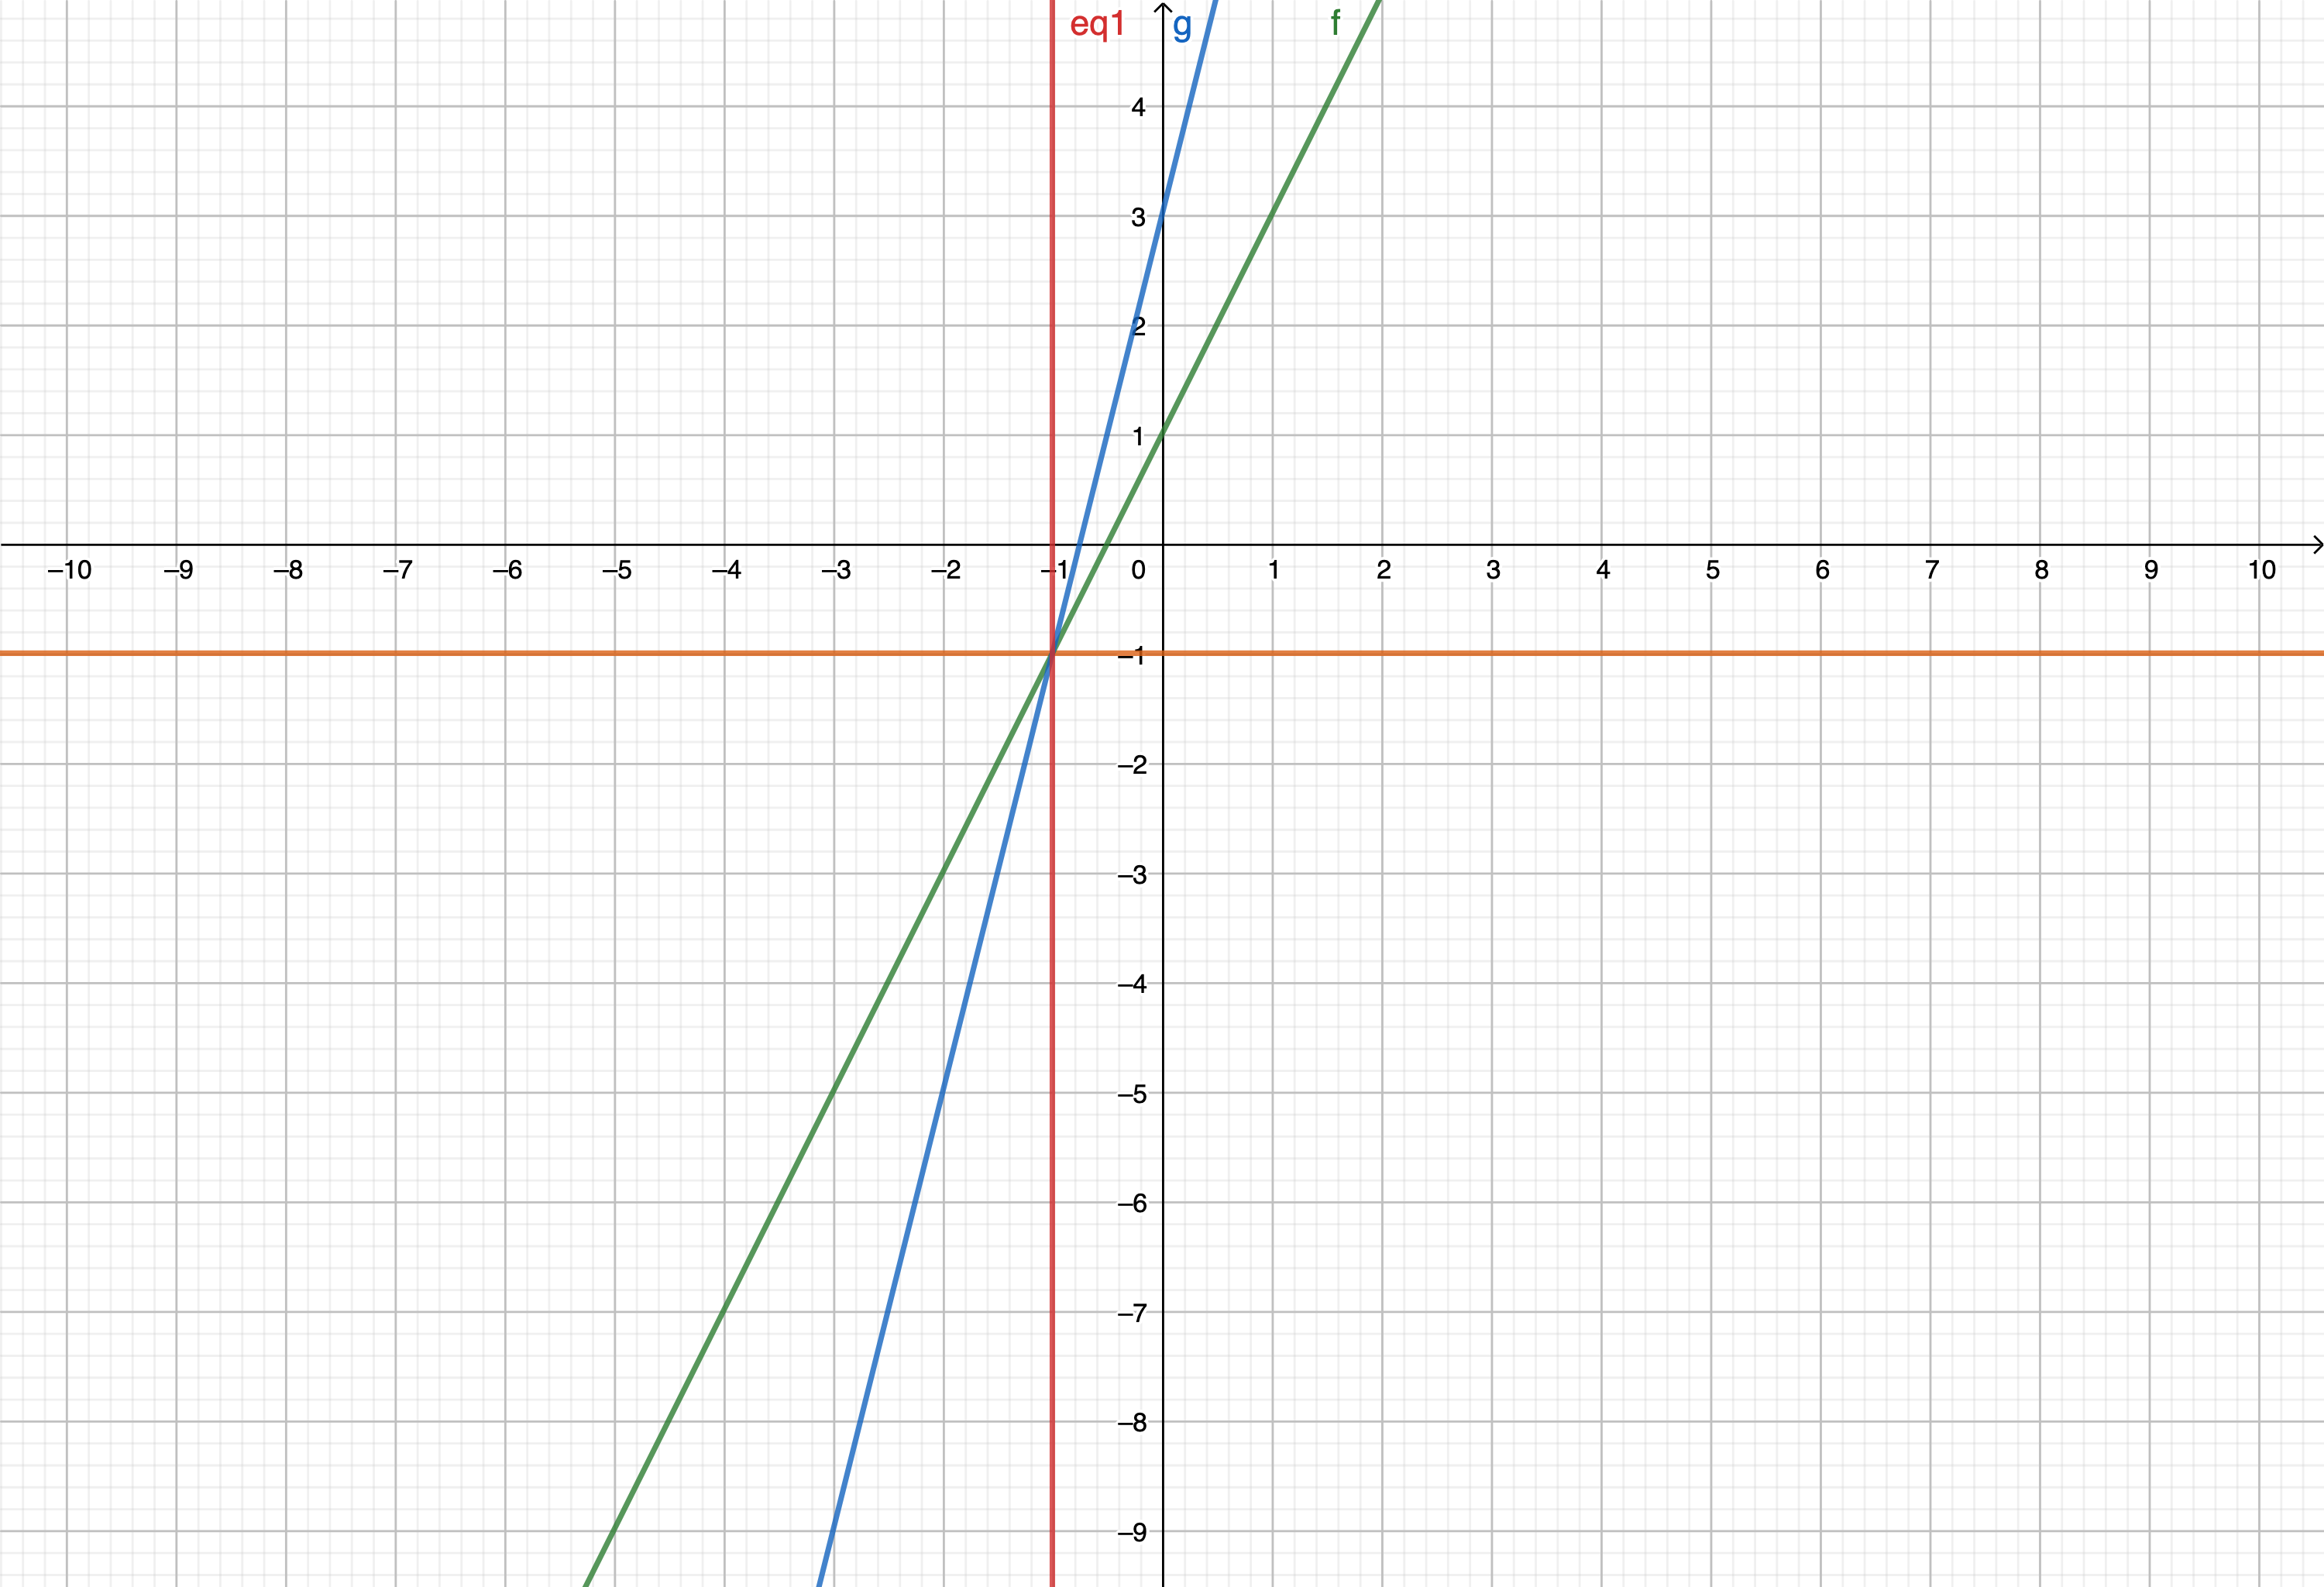
\includegraphics[scale=0.5]{epflLectureNotes/linearAlgebra/figures/linearGauss.png}
    \caption{Equivalent systems}
    \label{fig1}
\end{figure}

\subsubsection{Reducing a system to reduced row echelon form}

\begin{tcolorbox}
    \begin{align*}
     \text{Given} \left(\begin{matrix}0&3&-6&6&4&-5\\3&-7&8&-5&8&9\\3&-9&12&-9&6&15\end{matrix}\right)\\
     \text{We first realign to get} \left(\begin{matrix}3&-7&8&-5&8&9\\3&-9&12&-9&6&15\\0&3&-6&6&4&-5\end{matrix}\right) \\
     \text{After applying elementary row operations, we get the reduced row echelon form of}\\
     \left(\begin{matrix}1&0&-2&3&0&-24\\0&1&-2&2&0&-7\\0&0&0&0&1&4\end{matrix}\right)\\ 
     \text{Now anything which is not a pivot column is called a free variable.}\\
     x_{5} = 4\\
     x_{2} = 2x_{3} - 2x_{4} - 7\\
     x_{1} = 2x_{3} + 2x_{4} - 24
     \end{align*}
\end{tcolorbox}

\subsubsection{High school basics}

When solving systems of 2 unknowns or 3 unknowns, we simply are considering the system of lines or planes. Sticking to 3 dimensions, let's quickly recall how we obtain the formula's of a line and plane in 3-d. 
\\
A line in 3-d may be desribed in Vector form as:
\begin{equation*}
    l_[1] : \begin{bmatrix}
        A\\
        B\\
        C
    \end{bmatrix}
    + 
    \lambda\begin{bmatrix}
        D\\
        E\\
        F
    \end{bmatrix}
    +
    \psi\begin{bmatrix}
        G\\
        H\\
        I
    \end{bmatrix}
\end{equation*}

or may be simplified to cartesian form as: 
\begin{equation*}
    k = \frac{x + A}{B} = \ldots
\end{equation*}

Now, the equation of a plane is most commonly written in the form: 

\begin{equation*}
    Ax + By + Cz \ \text{where (A,B,C) is the normal vector to the plane.}
\end{equation*}

\section{Introducing vector spaces}
\subsection{Basics}
A vector space is an algebraic structure consisting of two sets, a scalar set and the vector set. The scalar set happens to be field and the vector set an additive abelian group. We also define a 'scalar multiplication' between the scalars and vectors to satisfy the following:

\begin{itemize}
    \item $r_{1}r_{2}(v_{1}) = (r_{1}r_{2})v_{1}$  \textbf{associativity of scalar multiplication}
    \item $r_{1}(v_{1}+v_{2}) = r_{1}v_{1}+ r_{1}v_{2}$ and the opposite as well, thus multiplication distributes over addition.
    \item $1_{r}v_{1} = v_{1}$
\end{itemize}

\begin{property}
From the above properties, we can neatly deduce also that $0_{r}v_{1} = 0$
\begin{align*}
    0_{r}v_{1} = (1-1)v_{1}\\
    1v_{1} - 1v_{1} = 0
\end{align*}
\end{property}
\\
The most common vector space is that of $\mathbb{R}^{n}$. It's vector and scalar set are the same. 
\subsection{Linear combinations,span and matrix theorems}

\begin{tcolorbox}
  A \textbf{linear combination} of vectors is simply a sum of vectors multiplied by scalars. 
  \begin{equation*}
      v_{i} = a_{1}v_{1} + \ldots + a_{k}v_{k}
  \end{equation*}
  A \textbf{span} for given vector set $\{v_{1}\ldots v_{k}\}$is simply a set that consists of all the possible outputs of $\sum_{i=1}^{k} a_{i}v_{i}$
\end{tcolorbox}

A common idea in linear algebra is to view a linear combination as the product of two matrices. We can't help but notice that:

\begin{equation*}
    a_{1}v_{1} + \ldots + a_{k}v_{k} = \begin{bmatrix}
        v_{1}  \ldots v_{k}
    \end{bmatrix} \begin{bmatrix}
        a_{1} \\
        \vdots \\
        a_{k}
    \end{bmatrix}
\end{equation*}

An important theorem that follows from the fact that $Ax=b$ is a set of equivalent statements(meaning they always have the same truth value.) 

\begin{thm}
\text{The following are equivalent:}
\begin{enumerate}
    \item $\forall b \in \mathbb{R}^{m}, Ax=b$ \text{has a solution}
    \item $ \forall b \in \mathbb{R}^{m}$ \text{b is a linear combination of the columns of A.}
    \item \text{columns of A span} $\mathbb{R}^{m}$
    \item \text{A(the coefficient matrix!) has a pivot position in each row. }
\end{enumerate}
\end{thm}

\subsection{Homogeneous system of equations}

Any system of linear equations that can be written of the form $Ax = 0$ is called \textbf{Homogeneous}. Clearly, this system has at least one solution which is when x is equal to the 0 vector. The non-trivial solution is if $x$ is not equal to 0 in which case the solution is described in terms of a parameter. Now, a theorem that follows is, for a non-homogeneous system $Ax=b$ with solution $p$, the solution set of $Ax=b$ is the set of vectors of the form $w = p + v_{h}$ where $v_{h}$ is any solution to $Ax = 0$.
\\ We now list some useful theorems. 
\begin{thm}
A homogeneous equation $Ax = 0$ has a nontrivial solution iff it has at least one free variable.
\end{thm}

\begin{thm}
Columns of A are linearly dependent iff $Ax=0$ has a trivial solution.
\end{thm}

\begin{thm}
Suppose the equation $Ax=b$ has a solution p. Then the set of possible solutions to $Ax=b$ are of the form $w = p + v_{h}$ where $v_{h}$ is a solution of $Ax = 0$.(Ofcourse assuming $Ax=b$ is consistent) That is to say, if we knew two solutions to $Ax=b$, we could find a solution to $Ax=0$. 
\end{thm}


\subsection{Linear Independence}
A set of vectors is linearly independent if the solution to:

\begin{equation*}
    a_{1}v_{1} + \ldots + a_{k}v_{k} = 0
\end{equation*}

is only the trivial solution, that is the $0_{v} \in \mathbb{R}^{k}$.
\\
We now present some common statements concerning linear independence. 
\begin{tcolorbox}
  \begin{thm}
    Whenever $Ax=0$ has a nontrivial solution, the columns of $A$ are linearly dependent. 
    \end{thm}
    
    \begin{thm}
    A set of vectors is linearly dependent if at least one of the vectors is a scalar multiple of the other.
    \end{thm}
    
    \begin{thm}
    If a set contains the zero vector, then it is linearly dependent.
    \end{thm}
    
    \begin{thm}
    If a set of vectors contain more vectors than vector entries, the set is linearly dependent.
    \end{thm}
    
    \begin{thm}
    A set of vectors is linearly dependent if the row echelon form of A to $Ax=0$ has at least one free variable.
    \end{thm}
    
\begin{thm}
\label{comb}
A set of vectors is linearly dependent iff at least one of the vectors can be written as a linear combination of the others.
\end{thm}

\begin{cor}
Two vectors are linearly dependent iff one is a scalar multiple of the other
\end{cor}

\end{tcolorbox}
Let's now prove the most useful out of these theorems. 

\begin{proof}
Let's first prove \ref{comb}.
\\
($\rightarrow$)
   Now suppose that for $S = \{ v_{1}, \ldots , v_{k}\}, v_{1} = a_{2}v_{2} + \ldots a_{k}v_{k}$ Then:
   $$ 0 = a_{2}v_{2} + \ldots - v_{1}$$
   In which case $v_{1}$ has a nonzero coefficient implying a nontrivial solution. 
   \\
($\leftarrow$)
Let $j$ represent the vectors that have a nonzero coefficient in $a_{1}v_{1} + \ldots + a_{j}v_{j} + \ldots a_{k}v_{k}$
\\
Now, WLOG, we get for all subscripts less than or equal to $j$:

$$ v_{1} = - \frac{a_{2}}{a_{1}}v_{2} - \ldots - \frac{a_{k}}{a_{1}}v_{k}$$
    \tag*{\qedhere}
\end{proof}

\subsection{Lec 05 notes}

\begin{property}
A linear $T$ maps linear line segments in $\mathbb{R}^{n}$ to linear line segments in $\mathbb{R}^{m}$ 
\end{property}

\subsubsection{Matrix transformations}

\begin{tcolorbox}
  In general, the columns of a matrix are the dimensions of the domain set and the rows of the matrix are the codomain. 
\end{tcolorbox}

\begin{thm}
Let $T$ be a square matrix, that is $T:\mathbb{R}^n \to \mathbb{R}^n$. Then, T is surjective iff it is injective. 
\end{thm}

\begin{proof} Proving both directions:
\\
($\rightarrow$) (T is injective iff T is surjective)
\\
Now whenever T is surjective, we have that there are no rows of 0. It also means that each row has a pivot. Given this, we check the condition that $T(v_{1}) = T(v_{2}) \rightarrow v_{1} = v_{2}$ Now we would essentially obtain this in trying to solve it:
\begin{equation*}
    T \times v = a
\end{equation*}
where $a \in \mathbb{R}^n$. Now because the reduced matrix has no 0 row and as many pivots as the number of variables, we get that there is only one such $v$ resulting in $v_{1} = v_{2}$
\\
($\leftarrow$) (T is surjective iff T is injective)
From $T$ is injective, we get that there is only one solution to $T \times v = a$ and considering the homogeneous $Tv=0$ we get that only 0 would be the solution implying columns of T are a basis hence must span $\mathbb{R}^n$
 \tag*{\qedhere}

\end{proof}

\subsection{Linear transformations}

\begin{definition}
A linear map is function between $\mathbb{R}^n \to \mathbb{R}^m$ such that:
\begin{align*}
    i) \ cT(v) = T(cv) \forall c \in \mathbb{R}, \forall v \in \mathbb{R}^n\\
    ii) \ T(v + u) = T(v) + T(u) \forall v,u \in \mathbb{R}^n
\end{align*}
\end{definition}

A condition equivalent to a linear map is:
\begin{prop}
Whenever we can show that for some $T$, $T(cv_{1} + dv_{2}) = cT(v_{1}) + dT(v_{2})$, we have that $T$ is a linear map.
\end{prop}

\begin{proof}(We must show both conditions i) and ii) defined above)
\\

Now showing i) is simple. Simply fix $d=0$. Then we get that $T(cv_{1} + 0) = cT(v_{1})$.
\\

To show ii), fix $c,d$ to be 1 and there we have it!

\end{proof}


\begin{thm}
For a linear transformation $T:\mathbb{R}^n \to \mathbb{R}^m$, there exists a unique $m\times n$matrix $A$ such that $T(x) = Ax$
\end{thm}

\begin{proof}
Now, we can write $x$ as $I_{n}x$ from which we get $\begin{bmatrix}
    e_{1} \ldots e_{n}
\end{bmatrix}x = x_{1}e_{1} + \ldots + x_{n}e_{n}$. Taking $T(x)$ we obtain $x_{1}T(e_{1}) + \ldots + x_{n}T(e_{n})$ which is equal to $$\begin{bmatrix}
    T(e_{1}) \ldots T(e_{n})
\end{bmatrix} \begin{bmatrix}
    x_{1} \\
    \vdots \\
    x_{n} 
\end{bmatrix}$$
\end{proof}

And here are some examples to capturing linear transforms as matrices mainly in $\mathbb{R}^2$
\begin{example}
\begin{enumerate}
    \item Anti-clockwise rotation by $\theta$ degrees. $A = \begin{bmatrix}
        \cos{\theta} & -\sin{\theta}\\
        \sin{\theta} & \cos{\theta}
    \end{bmatrix}$ 
    \item $T(x) = 3x$ for $x \in \mathbb{R} ^ 2$, then $A = \begin{bmatrix}
        3 & 0 \\
        0 & 3
    \end{bmatrix}$
    \item Reflection through the y-axis $A = \begin{bmatrix}
        -1 & 0\\
        0 & 1
    \end{bmatrix}$
    \item Contraction or an expansion depending on $k$ $ A = \begin{bmatrix}
        k & 0\\
        0 & 1
    \end{bmatrix}$ 
    \item Shear $\begin{bmatrix}
        1 & k\\
        0 & 1
    \end{bmatrix}$
    \item Projection $\begin{bmatrix}
        0 & 0\\
        0 & 1
    \end{bmatrix}$
    
\end{enumerate}
\end{example}


And now we present some theorems relating to surjectivity and injectivity:

\begin{thm}
Taking $T: \mathbb{R}^n \to \mathbb{R}^m$ we have that $T$ is injective iff the homogeneous $T(x) = 0$ has the trivial solution. 
\end{thm}

\begin{proof}(To show this, we show that the two statements always have the same truth value, that they are equivalent)

Now when $T(x)$ is injective, it means that $T(x) = 0$ can have only a unique solution by definition of injectivity. Now when $T(x)$ is not injective, it means that $\exists b$ s.t. $T(u) = b$ and $T(v) = b$ where $u \not = v$. Now $T(u) - T(v) = b-b = 0 = T(u-v)$ and since $u\not=v$ we have that $0$ is not the only solution.
\end{proof}

\section{Matrix algebra}

\subsection{Basics}

\begin{property}
Properties of the matrix transpose:
\begin{align*}
    (A^T)^T = A\\
    (A + B)^T = A^T + B^T\\
    (rA)^T = rA^T\\
    (AB)^T = B^TA^T
\end{align*}
\end{property}



\begin{property}
\begin{align*}
    A + B = B + A\\
    (A + B) + C = A + (B + C)\\
    A + 0 = A\\
    r(A + B) = rA + rB\\
    (r+s)A = rA + rS\\
    rs(A) = r(sA)
\end{align*}
\end{property}

And here is the general formula for the $i-j^{th}$ entry of $AB$ whenever defined:

$$(AB)_{ij} = a_{i1}b_{1j} + \ldots + a_{in}b_{nj}$$

\begin{remark}
We note that Matrices who's entries belong to $\mathbb{R}$ form a vector space.
\end{remark}

And now some warnings about matrix multiplication. We note that in general if $AB = AC$ then it does not hold that $B=C$ And if $AB=0$ we can not conclude that $A$ or $B$ is $0$. We also note that whenever a matrix has entries only along its main diagonal, then to take any power, we simply take the power of each diagonal entry. 
\\
A transpose of a matrix is defined as swapping the rows of $A$ with its columns. \\
\begin{thm}
A matrix $A$ is invertible if $\exists C$ s.t. $AC = I , CA=I$ meaning that the inverse is unique. Non-invertible matrices are called \textbf{singular}. And note that only square matrices are invertible. The reason for this is that for a matrix to be invertible, it must be bijective which can only be the case if it is square 
\end{thm}

\begin{proof}(Proving that the inverse matrix is unique)
Suppose $\exists B,C s.t. AB = I, \ AC=I$. We want to show that $B = C$.
\\
$B = BI = BAC = IC = C$
\end{proof}


\subsection{Computing inverses}

The way we find inverses is best done by Gaussian elimination. We are simply looking for a solution to the equation $Ax=I$ hence we write this as an augmented matrix $\begin{bmatrix}
    A | I
\end{bmatrix}$ and solve. 

\begin{thm}
\textbf{Elementary} matrices are obtained by only performing one elementary row operation on an identity matrix, thus all elementary matrices are invertible.
\end{thm}

\begin{thm}
Because inverses are only defined on bijective mappings, whenever a square matrix is invertible, we have that $Ax=b$ has a unique solution $x = A^{-1}b$
\end{thm}

\subsection{Every matrix is the product of elementary matrices with the identity}

Consider the matrix $E_{1}=$\begin{bmatrix}
    1 && 0 && 0\\
    0 && 1 && 0\\
    -4 && 0 && 1
\end{bmatrix} and $A=$ $E_{1}=$\begin{bmatrix}
    a && b && c\\
    d && e && f\\
    g && h && i
\end{bmatrix} Then notice that $E_{1}A=$ $E_{1}=$ \begin{bmatrix}
    a && b && c\\
    d && e && f\\
    g -4a && h -4b && i -4b
\end{bmatrix}

Which goes on to show that every row operation can be represented as the product of elementary matrices. 

\subsection{Characterizing inverse matrices}


 \begin{tcolorbox}[drop shadow, title=(Theorem on inverse matrices),lower separated=true]
    \centering
        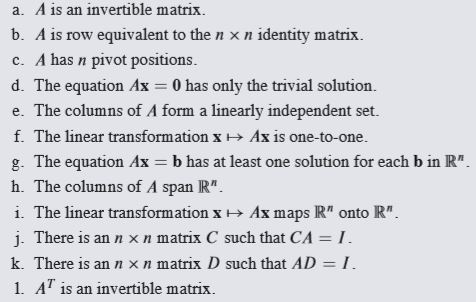
\includegraphics[scale = 0.9,valign=t]{epflLectureNotes/linearAlgebra/figures/invertible.JPG}
\end{tcolorbox}

\clearpage

\begin{figure}[H]
    \centering
    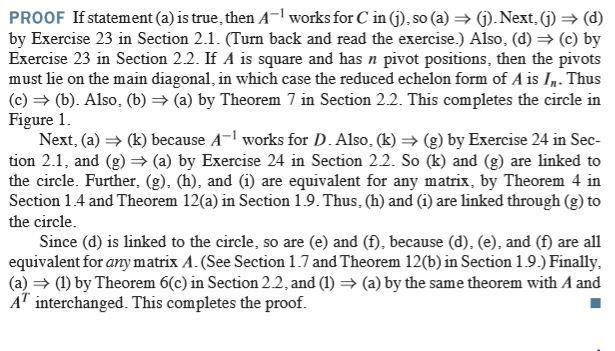
\includegraphics{epflLectureNotes/linearAlgebra/figures/proof.JPG}

\end{figure}

\section{Determinants}
\subsection{Basics}

First of all, determinant is only defined on an $nxn$ matrix and is denoted $det(A)$ or simply $|A|$
\\
The most useful formula for a determinant is 

$$ det(A) = \sum_{j=1}^{n} a_{1j}C_{1j}$$ or equivalently 
$$ det(A) = \sum_{i=1}^{n} a_{i1}C_{i1}$$
where $C_{ij}$ which is known as a \textit{cofactor} of matrix A is defined as:

$$ C_{ij} = (-1)^{i+j}det(A_{ij})$$ wherein $A_{ij}$ denotes a submatrix of A obtained by cancelling out the ith row and jth column of A. 
\\
Now the above formula is one way to calculate the determinant. An alternative method comes from the realization that whenever a matrix is triangular, its determinant is the product of the terms along its diagonal. Hence given a matrix $A$ we may row reduce it to its echelon form and simply find the product of all pivots. But noticing how 

$$ A = E_{1}\ldots E_{n}I$$ we get that

$$det(A) = det(E_{1})\ldots det(E_{n})$$

which means that because after row reduction we obtain $[I | A^{-1}]$, $det(A) = det(E_{1})\ldots det(E_{n}) \cdot det(I)$

This brings us to the following properties:

\begin{enumerate}
    \item If a multiple of one row is added to another to obtain matrix $B$, then $det(A) = det(B)$
    \item If a row is scaled by $k$ to obtain matrix $B$, then $det(B) = k \cdot det(A)$
    \item If two rows are interchanged, then $det(B) = -det(A)$
\end{enumerate}

\clearpage

And now a very important theorem is:

\begin{thm}
A matrix is $A$ invertible iff $det(A) \not = 0$ 
\end{thm}

\begin{proof}
When a matrix is invertible, we have that the solution to $Ax = 0$ is unique implying linear independence. And linear independence implies that $det(A) \not = 0$. 
\end{proof}

\begin{thm}
If $A$ is $nxn$, then $det(A^{T}) = det(A)$
\end{thm}

\begin{proof}
This is obvious. We have that the cofactors along the columns of $A^{T}$ are equal to cofactors of $A$ along rows and by definition of the transpose we have that $a_{1j} = a_{j1}$ which implies the coefficients are also equal. This also suggests why the earlier formula for $det(A)$ comes in two forms. 
\end{proof}

And now yet another theorem:

\begin{thm}
$det(AB) = det(A)det(B)$
\end{thm}


And now we come to Cramer's rule. It provides us with an alternative method for solving a system of equations using determinants. It states the following:

\begin{thm}(\textbf{Cramer's Rule})
\\
Where $A$ is an $n x n$ matrix, the solution to $Ax=b$ is of form 
$$x_{i} = \frac{|A_{i}(b)|}{|A|} \ i=1,2,3\ldots$$ 
where $A_{i}(b)$ is obtained by replacing the ith column of A with the vector b.
\end{thm}

\begin{proof}
Again quite simple. Notice that 

$$A\cdot I_{i}(b) = A[e_{1} \ldots b \dots e_{n}] = [a_{1} \ldots \underbrace{b}_{since Ax = b} \ldots a_{n}] = A_{i}(b)$$
Taking determinants we get $$det(A)\underbrace{det(I_{i}(b)}_{=x_{i}} = det(A_{i}(b)$$ to give $$ x_{i} = \frac{det(A_{i}(b))}{det(A)}$$
\end{proof}
\\
And now an important theorem is the following:

\begin{thm}
The area of the parallelogram determined by $a_{1}$ and $a_{2}$ is the same as that determined by $a_{1}$ and $a_{2} + ca_{1}$
\end{thm}

And furthermore:

\begin{thm}
For a linear transformation $T: \Rn \to  \Rn$ we have that whenever S is the generic shape in this vector space than the new area after T is given by:

$$ |T(s)| = |\det{A} \cdot |S|s$$
\end{thm}

\clearpage

\section{More on vector spaces}
\subsection{Basics}

\begin{tcolorbox}
\begin{definition}
A \textbf{Vector space} is an algebraic structure satisfying:

\begin{enumerate}
    \item For some vector set $V$ we have that $V$ is an abelian group under addition.
    \item Scalar multiplication between members of a scalar field and vector elements is defined and closure holds.
    \item Scalar multiplication of a vector associates
    \item $\forall v \in V$ we have that $1\cdot v = v$
    \item Multiplication of a scalar with two vectors distributes and multiplication of a vector with two scalars distributes. 
\end{enumerate}
\end{definition}
\end{tcolorbox}

Now three important facts that follow from these axioms are:

\begin{align}
    \label{1}0v = 0 \ \forall v \in V\\
    \label{2}c0 = 0 \ \forall c \in F\\
    \label{3}-u = (-1)u \ \forall u \in V
\end{align}

Let's prove these solely using the axioms. 
\begin{proof}
\\

\textbf{\ref{1}}
$$ 0v = (a-a)v = \underbrace{av - av}_{\text{\makebox[0pt]{additive inverse} }} = 0 $$

\textbf{\ref{2}}

$$ c0 = c(0-0) = c0 - c0 = 0$$

\textbf{\ref{3}}
\begin{align*}
    0u = (1-1)u\\
    0 = u + (-1)u\\
    -u = \underbrace{-u + u + (-1)u}_{\text{\makebox[0pt]{right additive inverse} }}
\end{align*}
\end{proof}


\begin{definition}
For a vector space $V$, $S$ is said to be a subspace if:

\begin{enumerate}
    \item $0_{v} \in S$
    \item $S$ is closed under scalar multiplication and vector addition
\end{enumerate}
\end{definition}

\begin{definition}(Null space)
\\
For some matrix $A$, the \textbf{Null space} is such that:
$$Nul A = \{v\in V| Av = 0_{v}\} $$
\end{definition}

\begin{prop}
$Nul A$ is a subspace of $V$
Now clearly $0 \in V$ as $0$ is the trivial solution to $Ax = 0$.
\\
We now need that $\forall u,v \in Nul A$, $u+v \in Nul A$.
$$A(u+v) = \underbrace{Au + Av}_{\text{\makebox[0pt]{matrices are linear maps}}} = 0 + 0 = 0$$
\\
We now also need $\forall u \in Nul A, \ cu \in A$

$$ A(cu) = cA(u) = c0 = 0$$
\end{prop}


\begin{thm}
The span of any single vector space elements is a subspace. 
\end{thm}

\begin{definition}(Column space)
\\
The column space $Col A$ is the set of all possible linear combinations of the columns of a matrix A and is also a subspace of $\mathbb{R}^{n}$ where $A:\mathbb{R}^{m} \to \mathbb{R}^{n}$.
\end{definition}


And now some examples of vector spaces:

\begin{example}
\begin{itemize}
    \item $\mathbb{R}^{n}$ is the most common example equipped with $\mathbb{R}$ as scalars.
    \item Set of polynomials of degree at most $n$ denoted $P_{n}$
    \item set of all real valued functions. This one is a little more subtle. Our 'vectors' are functions $f(x)$ and for instance the 0 vector is the map $g(x) = 0$. We define addition as $f(x) + g(x) = (f+g)(x)$ and scalar multiplication as $cf(x) = f(cx)$
\end{itemize}
\end{example}

Under light of vector spaces, a \textbf{linear transformation} is now much more clear as being a mapping that respects the two operations of vector spaces. 
\\

\subsection{Some problems from week 6}
\textbf{Claim:}
\\
Suppose matrix B is the reduced echelon form of the columns of $A$. Then the pivot columns of $B$ are a basis of $Col(A)$
\\

It is easy to see that this is false. Suppose $A$ is $\begin{bmatrix}
    1 && 0\\
    0 && 1\\
    0 && 1\\
\end{bmatrix}$ We then have that B is $\begin{bmatrix}
    1 && 0\\
    0 && 1\\
    0 && 0\\
\end{bmatrix}$ but clearly pivot columns of $B$ do not span $Col(A)$ 

\subsection{More theorems}

\begin{thm}
Let $S\subseteq V$ where $S$ is non-empty. And let $H = <S>$. Whenever one element of $S$ is l.d. on the other vectors, removing this element from $S$, we have that $S$ still spans $H$ And whenever $H \not = \{0_{v}\}$, some subset of $S$ is a basis for $H$. 
\end{thm}

\begin{thm}
The pivot columns of a matrix $A$ form a basis for $Col(A)$
\\
\textbf{Warning:} This does not mean that the pivot columns of the echelon form of $A$ are a basis to $Col(A)$ 
\end{thm}
\\

And now we come to a beatiful theorem of linear algebra, the unique representation theorem.

\begin{thm}
Any $v\in V$ is represented as the unique linear combination of the bases of $V$
\end{thm}

\begin{proof}
We have that:
$$ v = \sum_{i=0}^{k} a_{i}x_{i}$$
Now suppose also that:
$$ v = \sum_{i=0}^{k} b_{i}x_{i}$$

To give $$ \underbrace{v - v = 0}_{\text{\makebox[0pt]{additive inverse}}} = \sum_{i=0}^{k} a_{i}x_{i} - \sum_{i=0}^{k} b_{i}x_{i} = (a_{0} - b_{0})x_{0} + \ldots + (a_{k} - b_{k})x_{k}  $$
\\

Now since our $x_{i}$ are linearly independent only the trivial solution holds hence all $a_{i} - b_{i} = 0$ meaning that $a_{i} = b_{i}$
\end{proof}

\begin{definition}
Suppose $B = \{b_{1} \ldots\}$ is a basis for $V$ and $x \in V$. Then the \textbf{coordinates} of $x$ are simply weights $c_{i}$ such that $x =  \sum_{i=1}^{k} c_{i}b_{i}$ and are denoted $[x]_{b} = \begin{bmatrix}
    c_{1}\\
    \vdots \\
    c_{k}\\
\end{bmatrix}$
\end{definition}

\begin{exm}
(Change of coordinate matrix)
\\
The matrix equation 
$$ x = P_{b}x_{b}$$
transforms a vector $x$ with coordinates relative to $b$ into its coordinates in the standard bases. For instance suppose that $x = \begin{bmatrix}
    4 \\
    5\\
\end{bmatrix}$ and that $b_{1} = \begin{bmatrix}
    2 \\
    1 \\
\end{bmatrix}$ and $b_{2} = \begin{bmatrix}
    -1 \\
    1 \\
\end{bmatrix}$ Then $$ \begin{bmatrix}
    4 \\
    5\\
\end{bmatrix} =  c_{1}\begin{bmatrix}
    -1 \\
    1 \\
\end{bmatrix} + c_{2}\begin{bmatrix}
    2 \\
    1 \\
\end{bmatrix} = P_{b}x_{b} $$
Now crucially note that because $Col(P_{b})$ is a basis for $R^{n}$ we have that it is invertible.
\end{exm}

\begin{thm}(Basis conversion theorem)
To obtain coordinates of a given vector relative to some basis $B$ we do:

$$ [x]_{b} = P^{-1}_{b}x$$
\end{thm}

Another important property of vector spaces is that although for different bases, the coordinate vectors differ, a vector remains always the same. And now we come to present the coordinate mapping theorem. 

\begin{thm}(Coordinate mapping theorem)
\\ 
The vector $x$ is mapped to $[x]_{B}$. This is an example of a mapping from some random vector space onto $\mathbb{R}^n$ where $n = dim(V)$ From this we get that any finite-dimensional vector space has a linear bijection(aka. isomorphism) to $\mathbb{R}^n$ by simply using the coordinate mapping
\end{thm}

And another important theorem is the linear independence theorem:

\begin{thm}
If a vector space has a basis set with $n$ elements, then another set with more than $n$ elements has linearly dependent elements. 
\end{thm}

\begin{proof}
Let $\{u_{1} \ldots u_{p}\}$ be the set with more than $n$ vectors. Now we have that      
$$ c_{1}[u_{1}]_{B} + \ldots + c_{p}[u_{p}]_{B} = 0$$ has a non-trivial solution in $R^{n}$ since we have more vectors than entries. Now by linearity of the coordinate map we have:
$$ [c_{1}u_{1}]_{B} + \ldots + [c_{p}u_{p}]_{B} = 0$$ where at least one of the $c_{i}$ is not zero. 
\end{proof}


\begin{thm}
The dimension of $Nul(A)$ is the number of free variables to the equation $Ax=0$ which makes sense since every other vector in $Nul(A)$ is linearly dependent on a number of vectors equal to the number of free variables. The dimension of $Col(A)$ is the number of pivot columns 
\end{thm}

As an aside now, we state that differentiation of polynomials which generally maps $\mathbb{P}_{n} \to \mathbb{P}_{n}$ can be represented as a matrix transform. That is suppose $v \in \mathbb{P}_{2} = a_{0} + a_{1}x + a_{2}x^2$ Now we have that $T(v) = \dv{v}{x}$ The matrix mapping of this is:

$$ \begin{bmatrix}
0 && 1 && 0\\
0 && 0 && 2\\
0 && 0 && 0\\
\end{bmatrix}$$

\begin{definition}
The rank of a matrix $A$ is simply equal to $dim(Col(A))$
\end{definition}

A nice theorem making use of rank is:

\begin{thm}
If $A$ is an $m \cross n$ matrix then $A$ has rank 1 iff there are non-zero vectors $u \in \Rn$ and $v \in \Rm$ such that $A = uv^{T}$
\end{thm}

\begin{proof}
The forward direction says that given A with rank one, we have that any $i$ elements $\in Col(A)$ are linearly dependent. But notice that $uv^{T}$ is equivalent to:

$$ \begin{bmatrix}
    u_{1}\\
    \vdots\\
    u_{n}
\end{bmatrix} \begin{bmatrix}
    v_{1} && \hdots && v_{m}
\end{bmatrix}$$ which creates a matrix where every column is a scalar multiple of the other as the columns of $uv^{T}$ look like;
$$ v_{1}\begin{bmatrix}
    u_{1}\\
    \vdots\\
    u_{n}
\end{bmatrix},v_{2}\begin{bmatrix}
    u_{1}\\
    \vdots\\
    u_{n}
\end{bmatrix} \hdots$$
From this the backward direction trivially follows as well. 
\end{proof}

\subsection{Theorems of Rank, Col(A), Row(A) and Null(A)} 

\begin{tcolorbox}
\begin{thm}(Rank nullity theorem for matrices)
\\
This theorem states that for an $m\cross n$ matrix $A$:
$$ dim(Col(A)) + dim(Null(A)) = n$$
\end{thm}

\begin{proof}
Intuitively this should be obvious because $dim(Col(A))$ gives us the number of pivot columns in echelon form of $A$ and similarly any remaining columns give us the dimension of $Nul(A)$. Summing the two we get $n$. 
\end{proof}

\begin{thm} For a matrix $A$ with echelon form $B$, the row space of $A$ and $B$ are the same. The column space of $A$ has the same dimension as the column space of $B$ yet is not equivalent to it. However the column indices for which $B$ has pivot columns form a basis for $A$. 
\end{thm}
\end{tcolorbox}

\subsection{Change of basis}
Recall that we have already stated that every finite dimensional vector space is isomorphic to $\Rn$ through $x \to [x]_{B}$ known as the coordinate mapping. Given this coordinate mapping we know consider what it means to change basis.

\begin{exm}
Suppose that we have two bases $B_{i}$ and $C_{i}$ for some 2-dimensional $V$. And suppose that $b_{1} = 4c_{1}+c_{2}$ and $b_{2} = -6c_{1} + c_{2}$. Given that $[x]_{B} = \begin{bmatrix}
    3\\
    1
\end{bmatrix}$ we want to find $[x]_{C}$ Now we have:
$$ [x]_{B} = [3b_{1} + b_{2}]_{C} = 3[b_{1}]_{C} + [b_{2}]_{C} $$ which simplifies to the matrix multiplication:

$$ \begin{bmatrix}
    (b_{1})_{c} & (b_{2})_{C} 
\end{bmatrix}\begin{bmatrix}
    3\\
    1
\end{bmatrix} = [x]_{C}$$ 
\end{exm}

From this we obtain the change of basis formula which is:
$$ [x]_{C} = \underbrace{P_{B \to C}}_{\text{\makebox[0pt]{known as change of basis matrix}}}[x]_{B} $$

Now since the change of basis matrix is a non-zero square matrix, it follows that it is also invertible and in particular:

$$P_{B \to C}^{-1} = P_{C \to B}$$

\begin{exm}
Consider bases $B= \{ \begin{bmatrix}
    1\\
    1\\
    0
\end{bmatrix}, \begin{bmatrix}
    0\\
    1\\
    0
\end{bmatrix}, \begin{bmatrix}
    0\\
    0\\
    1
\end{bmatrix} \}$ and $C= \{ \begin{bmatrix}
    1\\
    2\\
    0
\end{bmatrix}, \begin{bmatrix}
    3\\
    2\\
    0
\end{bmatrix}, \begin{bmatrix}
    0\\
    0\\
    1
\end{bmatrix} \}$ And suppose that we want to find $P_{B\to C}$. Now this is equivalent to asking what the coordinate vectors of the basis $B$ are in the basis $C$. This result in having to solve 3 separate systems of the form:
$$ \begin{bmatrix}
    1\\
    1\\
    0
\end{bmatrix} = a\begin{bmatrix}
    1\\
    2\\
    0
\end{bmatrix} + b\begin{bmatrix}
    3\\
    2\\
    0
\end{bmatrix} + c\begin{bmatrix}
    0\\
    0\\
    1
\end{bmatrix}$$ which we simplify to the augmented matrix:

$$
  \begin{bmatrix}[ccc|ccc]
   1 & 3 & 0 & 1 & 0 & 0\\
   2 & 2 & 0 & 1 & 1 & 0\\
   3 & 0 & 1 & 0 & 0 & 1\\
\end{bmatrix}
$$
\end{exm}

We generalize our above example to that, to find $P_{B\to C}$ solve the matrix:

$$\begin{bmatrix}[c|c]
    P_{C} & P_{B}
\end{bmatrix} \rightarrow \begin{bmatrix}[c|c]
    I & P_{B\to C}
\end{bmatrix}$$

\subsection{Eigenvectors and eigenvalues}

\begin{definition}
An \textbf{eigenvector} of a square matrix is a vector such that $Ax$ can be written in form $\lambda x$ where $\lambda$ is a scalar. Of course when we state $Ax=\lambda x$, $x$ must be a non-trivial solution. 
\end{definition}

From the defining equation, we obtain that:
$$ (A - \lambda I)x = 0$$ and the set of all solutions belongs to the null space of the matrix $(A - \lambda I)$ and is called the $\textbf{eigenspace}$ of $A$ corresponding to $\lambda$. 

\begin{thm}
\label{eig}
The eigenvalues of a triangular matrix are the entries along its main diagonal.
\end{thm}

Now in general, what follows about determining if a matrix has an eigenvector is shown by the  following example:

\begin{property}
Suppose that $Ax = \lambda x$ where $x\not = 0_{v}$ Then it must follow that:
$$(A-\lambda I)x=0$$ has a nontrivial solution. Now since $A-\lambda I$ is a square matrix, we have that it will have a non-trivial solution $x$ iff. it's columns are linearly dependent. But note that this is equivalent to saying that $\det{A-\lambda I} = 0$ The fact the determinant is 0 iff. the matrix columns are \ld \ follows from the fact that the homogeneous equation of a square matrix in its echelon form will have at least one zero row to admit a nonzero solution and given that determinant of a triangular matrix is the product of entries in main diagonal we have that it will have determinant equal to zero. 
\end{property} 

\begin{thm}
If the matrix $(A-\lambda I)$ has no \ld \ columns than it has no eigenvectors. 
\end{thm}

Now note that we cannot use the equation $(A - \lambda I)=0$ to solve for $\lambda$
\\

Let's continue our exploration of eigenspaces noting that an eigenspace is a subspace of $V_{n}$:

\begin{exm}
Suppose $A = \begin{bmatrix}
    4 & -1 & 6\\
    2 & 1 & 6\\
    2 & -1 & 8 
\end{bmatrix}$ and we are given that $2$ is an eigenvalue of $A$. Now we have that $A - 2I = \begin{bmatrix}
    2 & -1 & 6\\
    2 & -1 & 6\\
    2 & -1 & 6 
\end{bmatrix}$ and in reduced homogeneous form we get:

$$  \begin{bmatrix}
    2 & -1 & 6 & 0\\
    0 & 0 & 0 & 0\\
     0 & 0 & 0 & 0
\end{bmatrix}$$ which gives a general solution: $x = y -6z$ and in parametric form: 

$$\begin{bmatrix}
    x\\
    y\\
    z
\end{bmatrix} = y\begin{bmatrix}
    1\\
    2\\
    0
\end{bmatrix} + z\begin{bmatrix}
    -3\\
    0\\
    1
\end{bmatrix}$$ Thus telling us also that the eigenspace for $2$ is a two-dimensional subspace of $\mathbb{R}^3$ Visually this is to say that matrix multiplication by $A$ has the same effect as scalar vector addition. 
\end{exm}

Given this, we now prove our earlier theorem \ref{eig}.
\begin{proof}
Note that a matrix has eigenvectors iff $A - \lambda I$ has determinant 0. Now determinant of a square triangular matrix is the entries along its diagonal hence we get:
$$(a_{11} - \lambda)(a_{22} - \lambda)(a_{33} - \lambda) = 0$$ which completes our proof.
\end{proof}
\\

And now we come to an interesting theorem of eigenvectors.

\begin{thm}
Suppose that for a square matrix $A$, $v_{i}$ are eigenvectors corresponding to eigenvalues $\lambda_{i}$. Then we have that the $v_{i}$ are \li .
\end{thm}

\begin{proof}
Now suppose that $p$ is the least index for which some $\underbrace{v_{p+1}}_{\text{\makebox[0pt]{$v_{i}$ are all nonzero$}}}$ can be written as a linear combination of vectors with smaller indices. Then we have that:

$$ v_{p+1} = a_{1}v_{1} + \ldots + a_{p}v_{p}$$ where at least one of the $a_{i} \not = 0$ Now using the fact that $Av_{k} = \lambda_{k}v_{k}$ we multiply the above by $A$ and replace the $Av_{k}$ to get:

$$ \lambda_{p+1}v_{p+1} = \lambda_{1}a_{1}v_{1} + \ldots + \lambda_{p}a_{p}v_{p} $$
As a final step we multiply our first equation with $\lambda_{p+1}$ and \underbrace{\text{subtract it from the above to get}}_{\text{\makebox[0pt]{our goal in doing is to obtain 0 on LHS}}}:

$$ a_{1}(\lambda_{1}-\lambda_{p+1})v_{1} + \ldots + a_{p}(\lambda_{p} - \lambda_{p+1})v_{p} = 0$$ Now because our $v_{i}$ up to $p$ are \li we have that the coefficients must all be 0. Since no $\lambda_{i} - \lambda_{i+1}$ can equal 0, we have that all of our $a_{i}$ must be 0. But then $v_{p+1}$ would be 0 which it cant be since it is an eigenvector.
\end{proof}

Now to present our next theorem we present the reminder that if we reduce square matrix $A$ to $U$ only using $r$ many row exchanges and row addition then:

\begin{empheq}[left =\text{$\det{A} = $}\empheqlbrace]{align*}
(-1)^{r}\det{U} \\
0 \ \text{if not invertible}
\end{empheq}



Now given our findings of eigenvectors we extend the invertible matrix theorem:
\begin{thm}(Extending invertible matrix theorem)
\begin{enumerate}
    \item $A$ is invertible iff. 0 is not an eigenvalue of $A$ This holds because than the echelon form of A will not have determinant 0 implying columns of A are \li
    \item $\det{A}$ is not 0. 
\end{enumerate}
\end{thm}

And this brings us to the characteristic equation theorem.

\begin{thm}(Characteristic equation theorem)
\\
$\lambda$ is a eigenvalue of square matrix $A$ iff. it satisfies:

$$\det{A-\lambda I} = 0$$ The expansion of $\det{A-\lambda I}$ is known as the \textbf{characteristic polynomial}. The \textbf{multiplicity} of some $\lambda$ value is in how many repeated roots $\lambda_{1}$ appears.
\end{thm}
\\

Moving on, two square matrices are said to be similar if both:
\begin{align*}
    P^{-1}AP = B\\
    PBP^{-1} = A
\end{align*}

The point of two matrices being similar is that whenever two matrices are similar, they essentially represent the same linear transformation between spaces however only in different bases.


\begin{thm}
If $A$ and $B$ are similar matrices, then they have the same characteristic polynomial hence the same eigenvalues. 
\end{thm}


\begin{thm}\textbf{(Representation of one matrix in another basis)}
\
Consider how we might represent one matrix in another basis $B$. That is suppose $A = \begin{bmatrix}
    -1 & 4 \\
    -2 & 3
\end{bmatrix}$ and we are given a basis $B = \{ \begin{bmatrix}
    3 \\
    2
\end{bmatrix}, \begin{bmatrix}
    -1 \\ 
    1
\end{bmatrix} \}$ Now it should be somewhat obvious that we must first apply the transformation to the bases and then find the coordinate of each result in the given basis. The matrix formed by these is then simply the coordinates of the bases $B$ after the transformation. Doing this follows as first finding the product $AB$ since for instance $A(\begin{bmatrix}
    3 \\
    2
\end{bmatrix}) = \text{first column of AB} = \begin{bmatrix}
    5 \\ 
    0
\end{bmatrix}$ And after we will have to solve $\begin{bmatrix}
    5 \\
    0
\end{bmatrix} = a \begin{bmatrix}
    3 \\ 
    2
\end{bmatrix} + b\begin{bmatrix}
    -1 \\ 
    1
\end{bmatrix}$ Formalizing this a little more we get that finding A in basis $B$ follows as solving:

$$\begin{bmatrix}[c|c]
    B & AB
\end{bmatrix} \rightarrow \begin{bmatrix}[c|c]
    I & A_{B}
\end{bmatrix}$$

In fact we can be even more formal. The matrix $A_B$ is nothing more than a matrix that takes as input a coordinate vector in basis $B$ and applies transformation $A$ on it. We obtain that:
$$A_{B} = \underbrace{B^{-1}}_{\text{\makebox[0pt]{obtain coordinates of bases after transformation}}}AB$$
\end{thm}


\begin{tcolorbox}
\textbf{Diagonilization, a useful computational tool}
\\

Now the first and foremost theorem of diagonilization is:
\begin{thm}
An $n\times n$ matrix $A$ is diagonilizable iff. it has $n$ linearly independent eigenvectors.
\end{thm}

\begin{proof}
We claim that $AP = PD$. Now $$AP = A\begin{bmatrix}
    v_{1} & \ldots & v_{n}
\end{bmatrix}$$ and similarly $$PD = P\begin{bmatrix}
    \lambda_{1} & 0 & \ldots & 0\\
    \0 & \lambda_{2} &  \ldots & 0$ \\
    \vdots & \ldots &  & \lambda_{n}\\
\end{bmatrix}$$

Now by vector equality we have that $Av_{i} = v_{i}\lambda_{i}$ Since now $P$ is an invertible matrix, we have that the $v_{i}$ are \li.
\end{proof}
\\

Now to diagonalize a matrix(ofcourse if possible only), we first find all eigenvalues by solving the characteristic polynomial. After we find the bases for each eigenvalue. Finally, $P$ is constructed as the matrix where each column is a basis corresponding to a respective eigenvalue found in the column vectors of matrix $D$.
\end{tcolorbox}


\subsection{Orthogonality and inner products}

\begin{definition}
Let $u,v \in \Rn$ Then we define the inner product of $u$ and $v$ as the matrix multiplication $u^{T}v$ such that $$ u \cdot v = u^{T}v = \begin{bmatrix}
    u_{1} \ldots u_{n}
\end{bmatrix}\begin{bmatrix}
    v_{1}\\
    \vdots\\
    v_{n}
\end{bmatrix} = u_{1}v_{1} + \ldots + u_{n}v_{n}$$ 
\end{definition}

\begin{definition}
The \textbf{norm} of a vector is defined in terms of inner product as $|v| = \sqrt{v\cdot v}$
\end{definition}

\begin{definition}
Distance in $\Rn$ is described by:
$$dist(u,v) = |u - v|$$
\end{definition}

\begin{definition}
$u$ and $v$ are orthogonal if $u\cdot v = 0$
\end{definition}

\begin{definition}
The orthogonal complement of some subspace $L$ is denoted $W^{\perp}$. It contains all vectors that are orthogonal to all vectors in $L$. 
\end{definition}

\begin{thm}$Row(A)^{\perp} = NulA$ and also $Col(A)^{\perp} = NulA^{T}$
\end{enumerate}
\end{thm}

\begin{proof}
For $Row(A)^{\perp} = NulA$, we have that every vector in $NulA$ has inner product $0$(aka. orthogonal) to every row of A. 
\\

For $Col(A)^{\perp} = NulA^{T}$ we use the fact that our above theorem is always true and given that $ColA = NulA^{T}$ we have $Col(A)^{\perp} = NulA^{T}$. 
\end{proof}

\begin{definition}
A set of vectors is an orthogonal set if each vector in the set is orthogonal to every other vector. Similarly, a \textbf{orthogonal basis} is a basis which is also an orthogonal set. 
\end{definition}

\begin{thm}
The usefulness of an orthogonal basis is in the fact that it is easy to find coordinates. We have that:
$$c_{i} = \frac{v \cdot u_{i}}{u_{i} \cdot u_{i}}$$
\end{thm}

\begin{proof}
$$v \cdot u_{i} = (c_{1}u_{1} + \ldots + c_{n}u_{n})u_{i} = c_{i}(u_{i}\cdot u_{i})$$
\end{proof}

\begin{definition}
A set is orthonormal if it is an orthogonal set of unit vectors. 
\end{definition}

\begin{thm}
An $m\times n$ matrix has orthogonal columns iff. $U^{T}U = I$
\end{thm}

And yet another useful theorem with its proof:
\begin{thm}
For $x,w \in \Rn$ and $A$ an $m\cross n$ matrix we have:
$w \cdot (Ax) = x \cdot (A^{T}w)$
\end{thm}

\begin{proof}
To see why this is true consider $U^{T}U$. Now this is equivalent to:

$$ \begin{bmatrix}
    \hdots u_{1} \hdots \\
    \hdots u_{2} \hdots \\
    \hdots u_{3} \hdots 
\end{bmatrix}\begin{bmatrix}
    u_{1} & u_{2} & u_{3}
\end{bmatrix}$$ Therefore it should be obvious that only the product of vectors with same indices should be the same producing the identity matrix. 

\end{proof}

\begin{proof}

$$ w\cdot(Ax) = \underbrace{(Ax)\cdot w}_{\text{\makebox[0pt]{by commutativity of dot product}} $$
$$ = (Ax)^{T}w = (x^{T}A^{T})w $$
$$ = x \cdot (A^{T}w)$$
\end{proof}

\begin{thm}
For a matrix with ortohonormal columns we have:
\begin{enumerate}
    \item $|Ux| = |x|$
    \item $(Ux)\cdot (Uy) = x\cdot y$
    \item $(Ux) \cdot (Uy) = 0$ iff. $x\cdot y =0 $
\end{enumerate}
\end{thm}

And now we come to a very useful theorem:

\begin{thm}\textbf{Orthogonal decomposition theorem}
\\

Let $y \in \Rn$. Then $y = y^{'} + z$ where:
$$ y^{'} = \frac{y \cdot u_{1}}{u_{1}\cdot u_{1}} + \ldots + \frac{y \cdot u_{p}}{u_{p} \cdot u_{p}}$$ with an orthogonal basis for $\{u_{1}, \ldots, u_{p}\}$ $W \leqslant \Rn$. And we also have that $z = y - y^{'}$
\end{thm}

\begin{proof}
Define a basis $\{u_{1}, \ldots, u_{p}\}$ for $W$. We then have that $$ y^{'} = \frac{y\cdot u_{1}}{u_{1}\cdot u_{1}}u_{1}+ \ldots + \frac{y \cdot u_{p}}{u_{p} \cdot u_{p}}u_{p}$$ Now we want to show that $z \in W^{\perp}$ For this to be true, $z$ must be orthogonal to all the basis vectors $u_{i}$. Given that $z = y - y^{'}$ we have that:
$$ (y-y^{'})\cdot u_{1} = y\cdot u_{1} - y^{'}u_{1} = y\cdot u_{1} - ( \frac{y\cdot u_{1}}{u_{1}\cdot u_{1}}u_{1}+ \ldots + \frac{y \cdot u_{p}}{u_{p} \cdot u_{p}}u_{p}) \cdot u_{1} = y\cdot u_{1} - y \cdot u_{1} = 0$$ By the very same argument, we have that $z$ is orthogonal to all the other $u_{i}$ hence we have that $z \in W^{\perp}$ 
\\

Finally we show uniqueness:

Suppose that $y = y^{'} + z$ and also that $y = x^{'} + w$ Then we have that:
$$ y^{'} + z = x^{'} + w $$ to further give: 

$$ y^{'} - x^{'} = w - z$$ which implies that $v = y^{'} - x^{'} \in W,W^{\perp}$ which is only possible if $v = 0$. This implies that $y^{'} = x^{'}$ and also that $w = z$. 
\end{proof}

And now comes a theorem about measurement in $\Rn$.

\begin{thm}
We have that:

$$|y-y^{'}| < |y - v| \ \text{for any $v$ distinct from $y^{'}$ and $y^{'}$ defined as $proj_{W}y$}$$
\end{thm}

\begin{proof}
We have that:

$$y-v = (y - y^{'})+(y^{'} - v)$$ and by the Pythagorean theorem we rather obviously have that:
$$ |y-v| > |y - y^{'}|$$
\end{proof}

\begin{thm}
Given that $U = \begin{bmatrix}
    u_{1} & u_{2} & \ldots & u_{p}
\end{bmatrix}$ and $U$ has orthonormal column vectors we have that:
$$y^{'} = UU^{T}y$$
\\

The above is clear considering that when we have an orthanormal basis $y^{'} = (y \cdot u_{1})u_{1} + \ldots$ that the weights $y \cdot u_{i}$ are equivalent to $u_{i}^{T}y$ which is equivalent to $U^{T}y$
\end{thm}

\begin{thm}
For a subspace $W$ of $\Rn$ we have that:
$$dim(W) + dim(W^{\perp}) = n$$
\end{thm}

\begin{proof}
Put the basis for $W$ and $W^{\perp}$ into one set. Now this is an orthogonal set which implies \li. Similarly, we have that every $y \in \Rn$ can be written as a linear combination of the elements in this set. Hence we are done.
\end{proof}

\begin{thm}\textbf{Uniqueness and existence theorem}
For some $Ax=b$ we have that the equality has a solution iff. $b\cdot y = 0 \ \forall y \in Nul(A^{T})$
\end{thm}

\begin{proof}
Firstly we have that $\Rn = \underbrace{W}_{\text{\makebox[0pt]{Col(A)}}} \bigoplus W^{\perp}$ and also that $b = y^{'} + z$ Now for $Ax=b$ to have a solution, we need that $b \in W$ this is only possible if $z = 0$ which implies that $\forall z \in Nul(A^{T})$ we have $b \cdot z = 0$ 
\end{proof}


\clearpage
\section{Factorizations and applications}
\begin{tcolorbox}\textbf{Gram-Schmidt}
We find an orthonormal basis for any vector space as follows:

Let $x_{i}$ form a basis. Now define:
\begin{align*}
    v_{1} = x_{1}\\
    v_{2} = x_{2} - \frac{x_{2}\cdot v_{1}}{v_{1}^2}v_{1}\\
    \ \vdots
\end{align*}

That is, the $v_{i}$ we find this way form an orthonormal basis. 
\\

\textbf{QR factorisation}
\begin{thm}
If $A$ is an $m\cross n$ matrix with \li \ columns we have that $A = QR$ where columns of $Q$ are an ortahonormal basis for $Col(A)$ and $R$ is upper triangular. 
\end{thm}

\begin{proof}
Now we have that $X =  A = \begin{bmatrix}
    x_{1} & \hdots & x_{n}
\end{bmatrix}$ Let $U = \begin{bmatrix}
    u_{1} & \hdots & u_{n}
\end{bmatrix}$ be the matrix with each column being an orthonormal vector.  Now by rewriting Gram-Schmidt we have that each $x_{i}$ is a linear combination of the $v_{i}$. Hence the matrix $R$ is the matrix simply containing these weights and we are done. 
\end{proof}
\end{tcolorbox}

\begin{definition}\textbf{Least squares problem}
When we try to estimate say a plot for some experiment data, the most natural approach is to minimize the distance between our chosen trendline and outlier experiment points. This generally leads to an equation of the form $b - Ax$ where our goal is to minimize this difference. For instance a polynomial estimation of degree 2 leaves us with:
$$ b - (a_{0} + a_{1}x^{1} + a_{2}x^{2}) = b - \begin{bmatrix}
    x^{0} & x^{1} & x^{2}
\end{bmatrix}\begin{bmatrix}
    a_{0}\\
    a_{1}\\
    a_{2}
\end{bmatrix}$$

Thus we have that a least squares solution is:

$$ |b - Ax^{'}| \leq |b - Ax| \ \forall x \in \Rn$$
\end{definition}

\begin{thm}\textbf{The general solution to the least squares problem}
This turns out to be the projection of the vector $b$ onto the columns space of $A$. Given that $b = b^{'} + z$ we have that $b - b^{'}$ is orthogonal to the column space of $A$ which implies $A^{T}(b-Ax) = 0$ Thus we conclude that the least square solution must always satisfy:
$$A^{T}b = A^{T}Ax$$
\end{thm}

Thus the general way to find a least squares solution is to solve for $x$ by finding $(A^{T}A)^{-1}A^{T}b$. Yet we note that this is only the case if $A^{T}A$ is invertible which happens when \textbf{the columns of $A^{T}A}$ are invertible.}
\\ 

Finally, if our $A$ happens to have linearly independent columns then the least squares solution to $Ax = b$ is even easier to find. We have that $A = QR$ and given that for orthanormal matrices $Q^{T} = Q^{-1}$ we get:
$$ x^{'} = R^{-1}Q^{T}b$$

\begin{thm}
\label{ort}
If $A$ is a symmetric matrix, then any two eigenvectors from a different eigenspace are orthagonal. 
We omit the proof but the idea is to consider $\lambda_{1}v_{1}\cdot v_{2}$ get that it is equal to  $\lambda_{2}v_{1}\cdot v_{2}$ and conclude.

\textbf{By the same idea we know that $A$ and $A^{T}$ have the same eigenvalues and we obtain that any two eigenvectors from a different eigenspace are orthogonal.}
\end{thm}

\begin{thm}
A square matrix $A$ is orthogonally diagonilizable that is $P$ being an orthogonal matrix iff. $A$ is symetric.
\end{thm}

\begin{remark}\textbf{Matrix multiplication can be viewed as a series of outer products}
We define an outer product as:
$$ x\tens{} y = xy^{T}$$
\end{remark}

\begin{tcolorbox}
\textbf{A useful tool: Spectral decomposition}
\\

Given our above theorem, we have that if $A$ is square and symetric, then it is orthogonally diagonilizable. So let $A = PDP^{-1}$. Taking $P$ to be an orthanormal matrix we obtain $A = PDP^{T}$ Now this simplifies to:
$$\begin{bmatrix}
    u_{1} & \hdots & u_{n}
\end{bmatrix}\begin{bmatrix}
    \lambda_{1} & \hdots
\end{bmatrix} \begin{bmatrix}
    u_{1}^{T}\\
    \vdots \\
    u_{n}^{T}
\end{bmatrix}$$
to finally give:
$$A = \lambda_{1}u_{1}u_{1}^{T} + \hdots + \lambda_{n}u_{n}u_{n}^{T} = \sum_{i=1}^{n}\lambda_{i}u_{i} \tens{} u_{i}$$
\end{tcolorbox}

\begin{definition} \textbf{Quadratic form}
\\
A quadratic form is a function that maps $\Rn$ to $\mathbb{R}$ and is of form $Q(x) = x^{T}Ax$ where $A$ is a square symetric matrix. For instance if $A = \begin{bmatrix}
    4 & 3\\
    3 & 2
\end{bmatrix}$ then $Q(x) = 4x^{2} + 6xy + 2y^{2}$ 
\end{definition}

We may also introduce the change of variable $x = Py$ where we represent our vector in $\Rn$ relative to some other basis in columns of $P$ and $y$ the coordinate vector in this basis. Then we have:
\begin{align*}
    x^{T}Ax\\
    (Py)^{T}APy\\
    y^{T}(P^{T}AP)y
\end{align*}
Now since A is a symetric matrix, by \ref{ort} we have that there is a diagonal matrix $D = P^{T}AP$ hence $x^{T}Ax = y^{T}Dy$ meaning that our quadratic form may be expressed without a cross product term. 


\begin{thm}\textbf{Principal axis theorem}
Our above result is now formalized to state that every quadratic form has a change of variable $x = Py$ such that $x^{T}Ax = y^{T}Dy$ where the second term has no cross product terms in it. Note that to find a principal axis, because we know that $A$ is symetric, it has an orthogonal diagonilazation hence we find out $D$ which is the matrix with eigenvalues as column entries. Then $P$ which is the principal axis is simply the matrix with eigenvectors corresponding the each eigenvalue. 
\end{thm}


\begin{definition}
Q(x) is positive definite if $>0$ negative definite of $<0$ and indefinite if both for $x \in \Rn$
\end{definition}

\begin{thm}
$Q(x)$ is positive definite iff. all eigenvalues of $A$ are positive (resp. definite). This is clear given that:

$$x^{T}Ax = y^{T}Dy = \lambda y_{1}^{2} + \ldots $$
\end{thm}


\begin{definition}\textbf{Constrained optimization}
Suppose we want to find a maximum value to the quadratic form $Q(x) = 9x^2 + 4y^2 + 3x^3$ with the constraint that our solution is a unit vector that is with $X = \begin{bmatrix}
    x \\
    y \\
    z
\end{bmatrix}$ and $|X^{T}X| = 1$. Since:
$$  9x^2 + 4y^2 + 3x^3 \leq 9(x + y + z) = 9$$ and since $Q(x) = 9$ has a solution, 9 is our maximum. 
\end{definition}


\begin{thm}
\label{eigenvalthm}
Let $A$ be a symmetric matrix and define:
$$ m = min\{x^{T}Ax: |x| = 1\} \ M = max\{x^{T}Ax: |x| = 1\}$$
Then we have that $m$ is the smallest eigenvalue of $A$ and $M$ the largest eigenvalue of $A$. 
\\

With eigenvalues $a \geq b \geq c$ as eigenvalues, the idea of the proof is to consider that $|x| = |y|$ then write out $y^{T}Dy = ay_{1}^{2} + by_{2}^{2} + cy_{3}^{2} \leq  ay_{1}^{2} + ay_{1}^{2} + ay_{1}^{2} = a(|y|) = a$ hence $M \leq a$ but clearly with $y = \begin{bmatrix}
    1\\
    0\\
    0
\end{bmatrix}$ hence $a = M$
\end{thm}

\begin{thm} In the previous case, our only constraint was that $|x| = 1$ namely that $x^{T}x=1$. Now if we add also that $x^{T}u_{1}=0$ meaning that the first component of $x$ is 0. Then it follows that the maximum possible value with this constraint is the second largest eigenvalue. Clearly than if we also add $x^{T}u_{2}=0$ the largest value becomes the third eigenvalue and so on. 
\end{thm}

\begin{thm}
$A^{T}A$ is symmetric. 
\end{thm}

\begin{thm}
In our previous case, we had that $A$ was symmetric hence finding a maximum was easy because we could always find a principal axis $P$ that led to $x^{T}Ax = y^{T}Dy$ making it easy to find a maximum. Now however, we consider the case where $A$ is not symmetric and we still want to find a maximum. Ie. such a mapping is the matrix that maps the unit sphere to some ellipse. We notice that the maximum of $|Ax|$ also maximises $|Ax|^{2}$ which is much easier to study as  $|Ax|^{2} = (Ax)^{T}(Ax) = x^{T}A^{T}Ax$ and fortunately, $A^{T}A$ is always square which means we can apply \ref{eigenvalthm} and know that the greatest eigenvalue $\lambda_{i}$ is the greatest value of $|Ax|^{2} = x^{T}A^{T}Ax$. Thus we obtain that the greatest value of a non-symmetric $Ax$ is given by $\sqrt{\lambda}$ and the $x$ satisfying this value, that is the element in the domain is any eigenvector $v_{i}$ with eigenvalue $\lambda_{i}$ Hence, we say that a \textbf{singular value} of $A$ is $|Av_{i}|$
\end{thm}


\begin{thm}
Suppose that for $A$ of dimension $m \cross n$, $v_{1}, \hdots, v_{n}$ is an orthogonal basis for $\Rn$ where each $v_{i}$ is an eigenvector of $\lambda_{i}$ where the $\lambda_{i}$ are eigenvalues of $A^{T}A$. Now, when $A$ has $r$ non-zero singular values, that is $r$ times next maxima, we have that $\{Av_{1}, \hdots, Av_{r}\}$ are a basis for $Col(A)$ and that $rank A = r$.
\end{thm}

\begin{thm}\textbf{Singular value decomposition}
When we have an $m\cross n$ matrix $A$ with rank $r$, we may write it as $U\Sigma V^{T}$ where $\Sigma$ is the diagonal matrix with $r$ many eigenvalues of $A$ in decreasing order. By considering $A^{T}A = V\Sigma^{T}\Sigma V^{T}$, we see that the entries of $\Sigma$ are also singular values of $A$.  
\end{thm}

\begin{remark}
Here is how we proceed to find the unique singular value decomposition.

\begin{enumerate}
    \item Find non-zero eigenvalue of $A^{T}A$.
    \item Construct $\Sigma$ diagonally from these eigenvalues not forgetting to take square-root!
    \item Construct each column of $V^{T}$ as eigenvectors corresponding to columns of $\Sigma$ where each eigenvector has as eigenvalue the square of singular values of $A$.
    \item Finally, columns of $U$ are $Av_{i}$ and we are done!
\end{enumerate}
\end{remark}









\end{document}
